\documentclass[10pt]{beamer}

\usepackage{appendixnumberbeamer}

\usepackage{booktabs}
\usepackage[scale=2]{ccicons}

\usepackage{pgfplots}
\usepgfplotslibrary{dateplot}

\usepackage{xspace}
\usepackage{../theme_style}
\setbeameroption{show notes on second screen}

\title[Synchronization]{Exam question one - Synchronization}
\subtitle{Distributed and Pervasive Systems}
\date{June 03, 2022}
\author[M.H. Kristensen]{Morten Haahr Kristensen}
\def\studentid{201807664}
\institute{Department of Electrical and Computer Engineering - Aarhus University}
% Logo only on title page
\titlegraphic{
    
\includegraphics[width=12cm]{figs/aulogo_big.png}
}
\begin{document}

\maketitle

\begin{frame}{Outline}
  \setbeamertemplate{section in toc}[sections numbered]
  \tableofcontents[hideallsubsections]
\end{frame}

\section{Motivation}

\begin{frame}{Motivation}
  \metroset{block=fill}
  \begin{alertblock}{Distributed System definition\cite{vansteenDistributedSystems2018}}
    A distributed system is a collection of autonomous computing elements that \textbf{appears} to its users as \textbf{a single coherent system}.
  \end{alertblock}
  \begin{itemize}
    \item Clock synchronization is related to coordination.
    \item Many distributed systems rely in one way or another on the notion of time.
    \begin{itemize}
      \item Can be real or logical time.
    \end{itemize}
    \item To appear as a single coherent system they must agree on the state i.e. the \textbf{current time.}
    \begin{itemize}
      \item They must also agree on the \textbf{ordering} of events.
    \end{itemize}
  \end{itemize}
\end{frame}

\begin{frame}{Example}
  \begin{figure}
    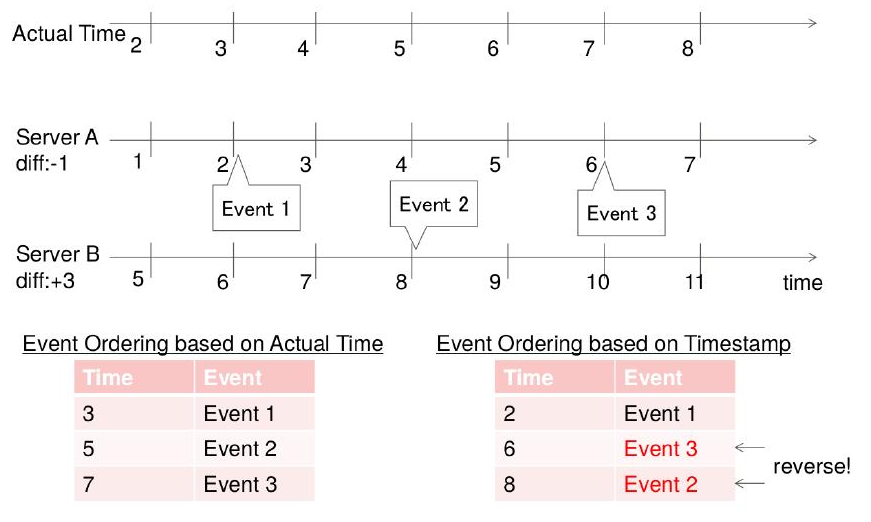
\includegraphics[width=\textwidth]{figs/bad_synchronization_example.png}
    \caption{Example of DS with bad clock synchronization.\cite{pedersenSynchronizationDistributedPervasive2022}}
  \end{figure}
\end{frame}

\section{Logical Clocks}

\begin{frame}{Definition}
  \textbf{Goal:}\qquad Chronological event ordering across nodes.\\
  \textbf{Context:}
  \begin{itemize}
    \vspace*{-0.2cm}
    \item Used when we are more interested in the \textbf{ordering} of events than knowing \textit{when} an event occurred.
    \item Processes keep track of local and global time.
    \begin{itemize}
      \item Updates local time after each local event.
      \item Updates global time after each data exchange.
    \end{itemize}
    \item Captures the causal relationships of events between processes.\note[item]{Events are causally related if one event may influence the outcome of another event.}
    \begin{itemize}
      \item If there is no causal relationship between two events they are considered to be happening concurrently.
    \end{itemize}
  \end{itemize}
\end{frame}

\begin{frame}{Lamport timestamps}
  \begin{itemize}
    \item Provides \textbf{partial ordering} in a distributed system.
    \note[item]{The result of partial ordering is that we cannot make sure that processes are synchronized before they start communicating. A process may be in an isolated state from the rest of the system.}
    \note[item]{''If two processes do not interact, it is not necessary that their clocks be synchronized because the lack of synchronization would not be observable and thus could not cause problems.''\cite[p.~310]{vansteenDistributedSystems2018}}
    \item Counters are used for timestamping.
    \item Events increment the counter.
    \begin{itemize}
      \item \textit{Sending and receiving is an event.}
    \end{itemize}
    \item Timestamps are always included with messages.
    \item Receiver updates to the greater counter before incrementing.
  \end{itemize}
\end{frame}

\begin{frame}[fragile]{Lamport timestamp example}
\begin{pythoncode}
# Sender:
time += 1
send(Message, time)

# Receiver:
(msg, timestamp) = receive()
time = max(timestamp, time)
time += 1

# Event:
wait_until(temperature < 20)
heat_room()
time += 1
\end{pythoncode}
\end{frame}

\begin{frame}[fragile]{Happened-before relation}
  The $\rightarrow$ symbol means ''happened before''.\\
  It has the following properties:
  \begin{table}
    \begin{tabular}{@{} lr @{}}
      \toprule
      Transitive: & $\forall\, e_1,\,e_2,\,e_3:\quad e_1 \rightarrow e_2,\, e_2 \rightarrow e_3 \implies e_1 \rightarrow e_3$ \\
      Irreflextive: & $\forall\,e_i:\quad e_i \nrightarrow e_i$ \\
      Antisymmetric: & $\forall e_1,\,e_2,\; e_1 \neq e_2:\quad e_1 \rightarrow e_2 \implies e_2 \nrightarrow e_1$\\
      \bottomrule
    \end{tabular}
  \end{table}
  Lamport timestamps give the following guarantees:
  \begin{table}
    \begin{tabular}{@{} lr @{}}
      \toprule
      Clock consistency: & $e_1 \rightarrow e_2 \implies C(e_1) < C(e_2)$ 
      \note[item]{Clock consistency: If we know that event 1 happened before event 2 then the timestamp of event 1 is less than the timestamp of event 2.} \\
      Contrapositive: & $C(e_1) \geq C(e_2) \implies e_1 \nrightarrow e_2$ 
      \note[item]{Contrapositive: If we know that the timestamp of event 1 is greater than or equal to the timestamp of event 2, then that implies that event 1 did not happen before event 2. So it can either have happened after or concurrently with event 2.} \\
      \sout{Strong clock consistency:} & $C(e_1) < C(e_2) \implies e_1 \rightarrow e_2 $
      \note[item]{Strong clock consistency: If the timestamp of event 1 is less than the timestamp of event 2, then that implies that event 1 occurred before event 2. (We can now infer event occurrences based on the timestamps.)}
      \note[item]{Since Lamport timestamps do not hold the strong clock consistency we cannot say anything about the relationships between $e_1$ and $e_2$ by merely comparing their timestamps $C(e_1)$ and $C(e_2)$.}\\
      \bottomrule
    \end{tabular}
  \end{table}
  Notation: $e_i = \textrm{event i.} \quad C(e_i) = \textrm{timestamp at event i}$
\end{frame}

\begin{frame}{Vector clocks}
  \begin{itemize}
    \item Provides \textbf{partial ordering} in a distributed system.
    \item A system of $N$ processes consists of a vector of $N$ 
    logical clocks. One for each process.
    \note[item]{Note that vector clocks assume that it is known beforehand how many processes are in the system.}
    \note[item]{Perhaps a solution to this could be using a dictionary and when comparing to clocks you consider a missing key to be "0".}
    \item An internal event increments the process' clock by one.
    \item Sending a message also increments the sender's clock by one and it sends a copy of its vector.
    \item When receiving a message the receiver increments its own clock and updates the vector by the element-wise maximum of each clock.
  \end{itemize}
\end{frame}

\begin{frame}[fragile]{Vector clocks comparison I}
Code checks if the vector clock v is smaller than w.\footnote{Example is a slightly altered version of \cite{krzyzanowskiLogicalClocks2021}}
\note{So we are doing a strict check where for a vector to be smaller every element is it must be smaller than or equal to.\\
Strictly speaking we should also check if they were identical but if the algorithm is implemented correctly it should be guaranteed that they aren't.}
\begin{pythoncode}
is_smaller(v : List, w : List)
  for v_el, w_el in zip(v, w)
    if v_el > w_el
      return False
  return True
\end{pythoncode}
\end{frame}

\begin{frame}[fragile]{Vector clocks comparison II}
Code checks if the vector clock v is concurrent with w.\footnote{Example is a slightly altered version of \cite{krzyzanowskiLogicalClocks2021}}
\note{We can see from the code that concurrency checking is done by checking some of the elements are less than and others are greater than.\\
If it returns True then the events are concurrent. If not they are not concurrent.}
\begin{pythoncode}
is_concurrent(v : List, w : List)
{
  greater=False, less=False
  for v_el, w_el in zip(v, w)
    if v_el > w_el
      greater = true;
    elif v_el < w_el
      less = true;
  return greater and less
}
  \end{pythoncode}
Or as an unoptimized oneliner:\\
\pythoninline{return not is_smaller and not is_greater}
\end{frame}

\begin{frame}{Example Lamport}
  \begin{figure}
    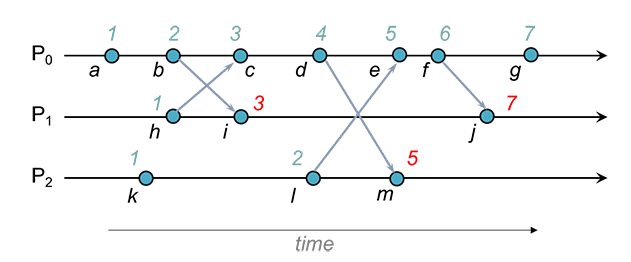
\includegraphics[width=\textwidth]{figs/lamport_timestamps.png}
    \caption{Example of Lamport timestamps.\cite{krzyzanowskiLogicalClocks2021}}
  \end{figure}
  \note{%
  \begin{itemize}
    \item We have three processes that each keep track of the Lamport timestamp.
    \item Event $b$ and $i$. If event $i$ was a normal timestamp it would get a value of 2. Since it received the timestamp 2 it increments it by 1 and sets the local time to 3.
    \begin{itemize}
      \item This preserves that $b \rightarrow i$
    \end{itemize}
    \item Event $c$ receives the message from event $h$. Here the timestamp is simply incremented by 1, since the timestamp at $h = 1 < 2$.
    \item We can say that event $h$ happened before event $m$ since $h \rightarrow c, c \rightarrow d, d \rightarrow m$ and the happened-before relation is transitive. 
    \item The timestamps reflects this. $h=1 < m=5$ but we cannot always conclude that based on the timestamps.
    \begin{itemize}
      \item E.g. $k = 1 < i = 3$ but $k$ did not happen before $i$. They happened concurrently. This is where normal clock consistency falls short.
    \end{itemize}
  \end{itemize}
  }
\end{frame}

\begin{frame}{Example Vector clocks}
  \begin{figure}
    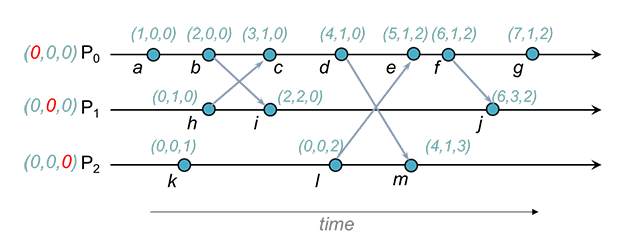
\includegraphics[width=\textwidth]{figs/vector_clocks.png}
    \caption{Example of vector clocks.\cite{krzyzanowskiLogicalClocks2021}}
  \end{figure}
  \note{%
    \begin{itemize}
      \item Events $b$ and $i$. If $i$ was a local timestamp it would get $(0, 2, 0)$. But it updates corresponding to $b$'s vector. Since they both have $0$ as the last element it is kept.
      \item Events $e = (5,1,2) < j = (6,3,2)$ since every element is less. The events are causally related: $e \rightarrow j$
      \item Events $f = (6,1,2)$ and $m = (4,1,3)$ are concurrent (that is not causally related). Because: $f1 > m1$ but $f3 < m3$.
    \end{itemize}
  }
\end{frame}

\section{Real Clocks}

\begin{frame}{When logical ordering isn't enough}
Many distributed systems require comparisons between external events

Allows for total ordering of events but comes with synchronization issues.

\textbf{Motivation by example:}\\
I want to know how much money I have spent \textit{since my birthday}.
\note{So in this small example we have a distributed banking system that uses logical clocks.\\
But suddenly the user puts wants to know how much money he has spent since the external event of his birthday.\\
We can't compare this to our logical clocks (partial ordering and all) so we need a new system.
Luckily, we learned of this system back in 1st grade.\\
Turns out that it is not that simple in a distributed system because the processes must agree on the time with a certain precision. And clocks drift over time.}

\vspace{1cm}
Different protocols to choose from. This course chooses \textbf{IEEE PTPv2}.\\
\textbf{Goal:} Provide sub $\mu s$ precision.
\end{frame}

\begin{frame}{IEEE Precision Time Protocol (PTP)}
  \begin{figure}
    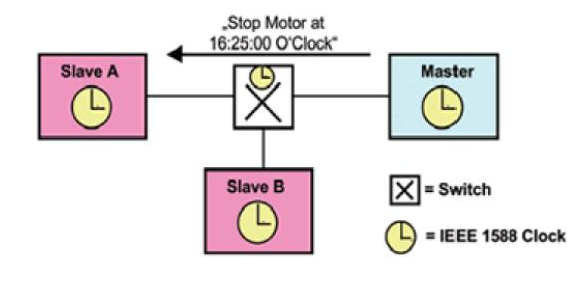
\includegraphics[width=\textwidth]{figs/ptp_clock_synchronization.png}
    \caption{Overview of PTP.\cite{pedersenSynchronizationDistributedPervasive2022}}
  \end{figure}
  \note[item]{%
    The main idea behind PTP is very simple. Assign a master and let it determine the system clock. The slaves synchronize to this clock in regards to offset and latency.
  }
  Where does the master get its clock from?
  \note[item]{%
      The protocol allows for the master clock to behave as a boundary clock. I.e. to our system, it is a master but to a greater system, it is a slave.\\
      Ideally, the master clock should be directly connected to the atomic clocks determining UTC.
  }
\end{frame}

\begin{frame}{PTP Phase 1: Offset correction}
  \begin{figure}
    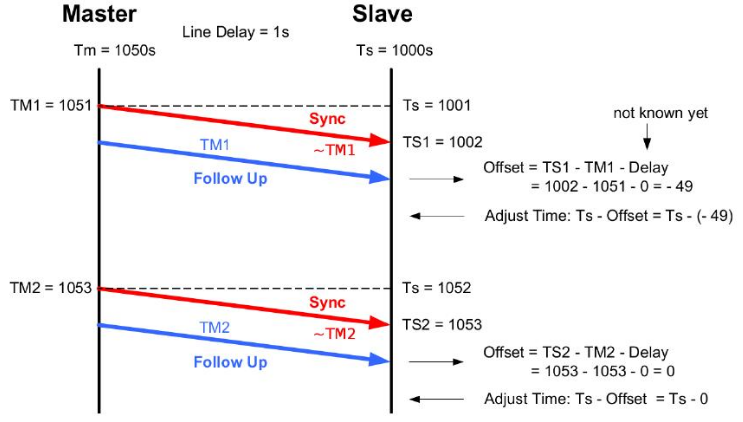
\includegraphics[width=\textwidth]{figs/ptp_phase1.png}
    \caption{Phase 1 of PTP.\cite{pedersenSynchronizationDistributedPervasive2022}}
  \end{figure}
  \centering 
  Assumes delay of 0s.
  \note{%
    This phase is also sometimes called syntonization.\\
    During the first phase, we take a naive approach and assume a delay between the master and slave of 0s.\\
    The master sends a sync request to the slave. The follow-up contains the actual timestamp (1051). (It is done this way to provide better accuracy as it is assumed that it takes time to generate the accurate timestamp). The slave compares the timestamp to its time to calculate the offset. $1002 - 1051 = -49$. The slave corrects its clock.\\
    The process is repeated until they agree on the time.
  }
\end{frame}

\begin{frame}{PTP Phase 2: Delay correction}
  \begin{figure}
    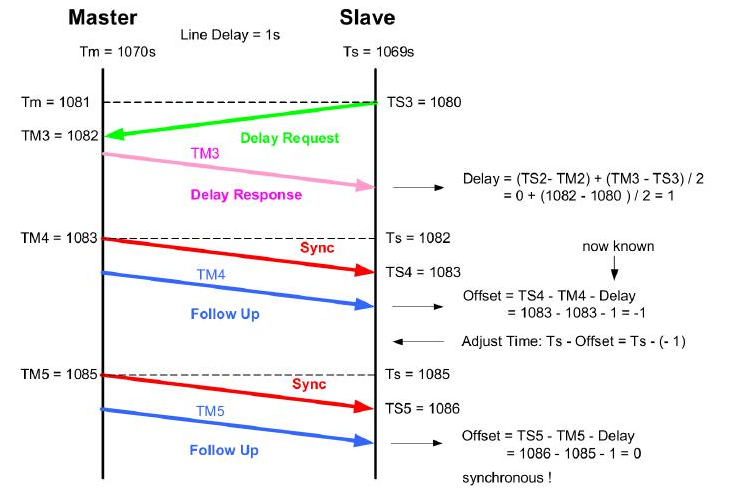
\includegraphics[width=0.95\textwidth]{figs/ptp_phase2.png}
    \caption{Phase 2 of PTP.\cite{pedersenSynchronizationDistributedPervasive2022}}
  \end{figure}
  \centering 
  Assumed symmetric delay.
  \note{%
    In this example, there is a delay of 1s each way.\\
    The slave sends a delay request to the master and the master returns a response with the current time.\\
    The slave can then find the delay based on the previous offset values and the time spent between the delay request and response. This turns out to be 2, so the final delay is 1.\\
    We can now repeat phase 1 to remove the offset again since the slave's clock is one second ahead. They are finally synchronous.\\
    If you have asynchronous delays you may need to fine-tune the division part. E.g. divide TM3 by 1.7 and TS3 by 2.3. (Or maybe more intuitively say TM3*0.4 and TS3*0.6).
  }
\end{frame}

\begin{frame}{Where to put the PTP layer?}
  \begin{figure}
    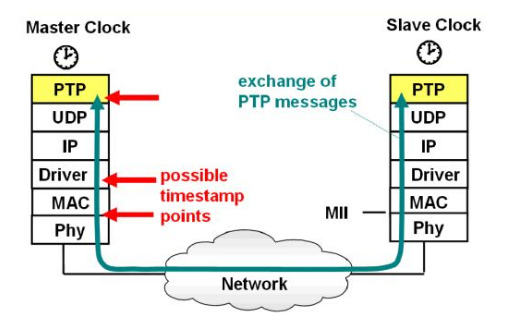
\includegraphics[width=0.95\textwidth]{figs/ptp_timestamp_generation.png}
    \caption{Network layer and PTP.\cite{pedersenSynchronizationDistributedPervasive2022}}
  \end{figure}
  \note{%
    One final note is where to put the PTP layer in terms of the network layer model.\\
    As the slide indicates it is possible to put PTP as the upper most layer where it is handled entirely by software.\\
    It is probably better to put it closer to the physical layer though as this can provide better precision.\\
    Depending on which kind of processor we are using, the delay for generating a timestamp may not be constant. Furthermore, most software stacks don't support timestamps of sub $\mu s$ precision.
  }
\end{frame}

\section{References}
\begin{frame}[allowframebreaks]{References}
  \bibliographystyle{ieeetr}
  \bibliography{references}
\end{frame}

\end{document}
